\documentclass[tikz,border=0pt,11pt]{standalone}
\usepackage[T1]{fontenc}
\usepackage[utf8]{inputenc}
\usepackage{lmodern,amsmath,amssymb}
\usepackage[swedish]{babel}
\usetikzlibrary{arrows.meta,calc,positioning,decorations.pathmorphing,decorations.pathreplacing,patterns,shadings}
\definecolor{navy}{HTML}{102F40}
\definecolor{teal}{HTML}{147D78}
\definecolor{lightteal}{HTML}{E6F1ED}
\definecolor{gold}{HTML}{B88B3B}
\definecolor{palegold}{HTML}{F7EEDB}
\definecolor{rust}{HTML}{B6533B}
\definecolor{palerust}{HTML}{FAEAE4}
\definecolor{paper}{HTML}{F7F5EE}
\definecolor{muted}{HTML}{5B6D72}
\definecolor{line}{HTML}{D6DED8}
\renewcommand{\familydefault}{\sfdefault}
\newcommand{\atom}[5]{\shade[ball color=#3!70] (#1,#2) circle (#5);\node[text=white,font=\bfseries\small] at (#1,#2){#4};}
\newcommand{\water}[3]{\begin{scope}[shift={(#1,#2)},scale=#3]\draw[navy!45,line width=2pt] (-.3,.22)--(0,0)--(.3,.22);\atom{0}{0}{rust}{O}{.22}\atom{-.3}{.22}{teal}{H}{.15}\atom{.3}{.22}{teal}{H}{.15}\end{scope}}
\newcommand{\panel}[4]{\filldraw[fill=white,draw=line,rounded corners=5pt] (#1,#2) rectangle ++(#3,#4);}
\newcommand{\note}[4]{\node[txt,text width=#3cm] at (#1,#2){#4};}
\tikzset{txt/.style={anchor=north west,align=left,text=navy,font=\small},
 head/.style={anchor=west,text=navy,font=\bfseries\large},
 label/.style={align=center,text=navy,font=\small},
 smalllabel/.style={align=center,text=muted,font=\footnotesize},
 arrow/.style={-{Latex[length=2.5mm,width=1.8mm]},line width=1.2pt,draw=teal},
 goldarrow/.style={-{Latex[length=2.5mm]},line width=1.2pt,draw=gold},
 rustarrow/.style={-{Latex[length=2.5mm]},line width=1.2pt,draw=rust},
 dashedarrow/.style={arrow,dashed},
 badge/.style={fill=lightteal,rounded corners=3pt,text=teal,font=\bfseries\small,inner sep=5pt}}
\begin{document}
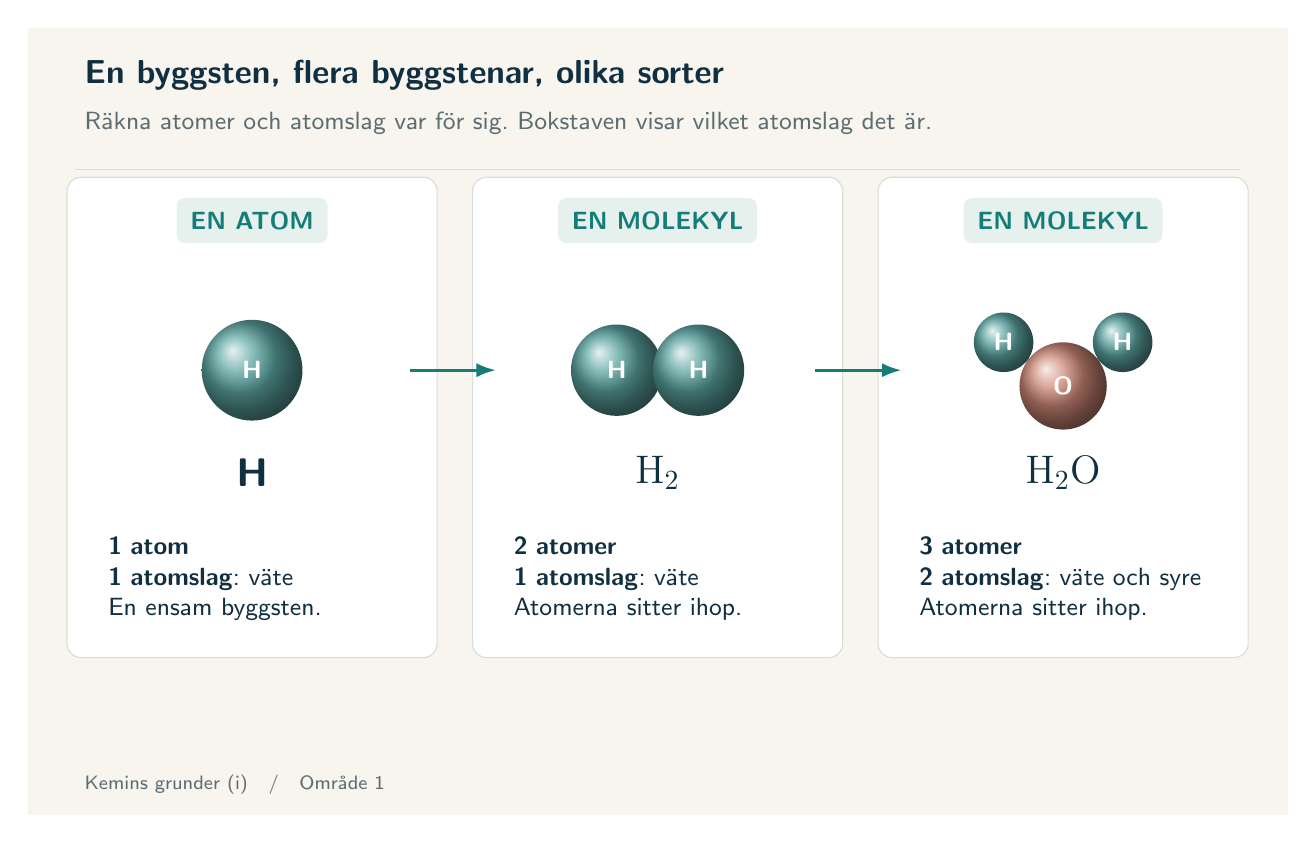
\begin{tikzpicture}[x=1cm,y=1cm]
\path[use as bounding box] (0,0) rectangle (16,10);
\fill[paper] (0,0) rectangle (16,10);
\node[head] at (.6,9.4){En byggsten, flera byggstenar, olika sorter};
\note{.6}{9.05}{14.8}{\textcolor{muted}{Räkna atomer och atomslag var för sig. Bokstaven visar vilket atomslag det är.}}
\draw[line] (.6,8.2)--(15.4,8.2);

\panel{.5}{2}{4.7}{6.1}\panel{5.65}{2}{4.7}{6.1}\panel{10.8}{2}{4.7}{6.1}
\node[badge] at (2.85,7.55){EN ATOM};\node[badge] at (8,7.55){EN MOLEKYL};\node[badge] at (13.15,7.55){EN MOLEKYL};
\atom{2.85}{5.65}{teal}{H}{.64}
\draw[navy!50,line width=4pt] (7.48,5.65)--(8.52,5.65);
\atom{7.48}{5.65}{teal}{H}{.58}\atom{8.52}{5.65}{teal}{H}{.58}
\begin{scope}[shift={(13.15,5.45)},scale=1.8]\water{0}{0}{1.4}\end{scope}
\node[label,font=\bfseries\Large] at (2.85,4.35){H};\node[label,font=\bfseries\Large] at (8,4.35){$\mathrm{H_2}$};\node[label,font=\bfseries\Large] at (13.15,4.35){$\mathrm{H_2O}$};
\note{.9}{3.65}{3.9}{\textbf{1 atom}\par \textbf{1 atomslag}: väte\par En ensam byggsten.}
\note{6.05}{3.65}{3.9}{\textbf{2 atomer}\par \textbf{1 atomslag}: väte\par Atomerna sitter ihop.}
\note{11.2}{3.65}{3.9}{\textbf{3 atomer}\par \textbf{2 atomslag}: väte och syre\par Atomerna sitter ihop.}
\draw[arrow] (4.85,5.65)--(5.95,5.65);\draw[arrow] (10,5.65)--(11.1,5.65);\node[anchor=west,text=muted,font=\scriptsize] at (.6,.38){Kemins grunder (i)\quad /\quad Område 1};

\end{tikzpicture}\end{document}
